

\documentclass[DM,authoryear,toc]{lsstdoc}
% lsstdoc documentation: https://lsst-texmf.lsst.io/lsstdoc.html

\input{meta}
% Package imports go here.

% Local commands go here.
% DO NOT EDIT - generated by /Users/womullan/LSSTgit/lsst-texmf/bin/generateAcronyms.py from https://lsst-texmf.lsst.io/.
\newacronym{AD} {AD} {Associate Director}
\newglossaryentry{AURA} {name={AURA}, description={\gls{Association of Universities for Research in Astronomy}}}
\newglossaryentry{Alert} {name={Alert}, description={A packet of information for each source detected with signal-to-noise ratio > 5 in a difference image during Prompt Processing, containing measurement and characterization parameters based on the past 12 months of LSST observations plus small cutouts of the single-visit, template, and difference images, distributed via the internet.}}
\newglossaryentry{Alert Production} {name={Alert Production}, description={The principal component of Prompt Processing that processes and calibrates incoming images, performs Difference Image Analysis to identify DIASources and DIAObjects, packages and distributes the resulting Alerts, and runs the Moving Object Processing System.}}
\newglossaryentry{Archive} {name={Archive}, description={The repository for documents required by the NSF to be kept. These include documents related to design and development, construction, integration, test, and operations of the LSST observatory system. The archive is maintained using the enterprise content management system DocuShare, which is accessible through a link on the project website www.project.lsst.org.}}
\newglossaryentry{Archive Center} {name={Archive Center}, description={Part of the LSST Data Management System, the LSST archive center is a data center at NCSA that hosts the LSST Archive, which includes released science data and metadata, observatory and engineering data, and supporting software such as the LSST Software Stack.}}
\newglossaryentry{Association Pipeline} {name={Association Pipeline}, description={An application that matches detected Sources or DIASources or generated Objects to an existing catalog of Objects, producing a (possibly many-to-many) set of associations and a list of unassociated inputs. Association Pipelines are used in Prompt Processing after DIASource generation and in the final stages of Data Release processing to ensure continuity of Object identifiers.}}
\newglossaryentry{Association of Universities for Research in Astronomy} {name={Association of Universities for Research in Astronomy}, description={ consortium of US institutions and international affiliates that operates world-class astronomical observatories, AURA is the legal entity responsible for managing what it calls independent operating Centers, including LSST, under respective cooperative agreements with the National Science Foundation. AURA assumes fiducial responsibility for the funds provided through those cooperative agreements. AURA also is the legal owner of the AURA Observatory properties in Chile.}}
\newglossaryentry{CCD} {name={CCD}, description={\gls{Charge-Coupled Device}}}
\newglossaryentry{Center} {name={Center}, description={An entity managed by AURA that is responsible for execution of a federally funded project}}
\newglossaryentry{Charge-Coupled Device} {name={Charge-Coupled Device}, description={a particular kind of solid-state sensor for detecting optical-band photons. It is composed of a 2-D array of pixels, and one or more read-out amplifiers.}}
\newglossaryentry{Commissioning} {name={Commissioning}, description={A two-year phase at the end of the Construction project during which a technical team a) integrates the various technical components of the three subsystems; b) shows their compliance with ICDs and system-level requirements as detailed in the LSST Observatory System Specifications document (OSS, LSE-30); and c) performs science verification to show compliance with the survey performance specifications as detailed in the LSST Science Requirements Document (SRD, LPM-17).}}
\newglossaryentry{Construction} {name={Construction}, description={The period during which LSST observatory facilities, components, hardware, and software are built, tested, integrated, and commissioned. Construction follows design and development and precedes operations. The LSST construction phase is funded through the \gls{NSF} \gls{MREFC} account.}}
\newacronym{DESC} {DESC} {Dark Energy Science Collaboration}
\newglossaryentry{DIASource} {name={DIASource}, description={A DIASource is a detection with signal-to-noise ratio greater than 5 in a difference image.}}
\newacronym{DM} {DM} {\gls{Data Management}}
\newacronym{DMS} {DMS} {Data Management Subsystem}
\newglossaryentry{DMTN} {name={DMTN}, description={DM Technical Note}}
\newacronym{DR} {DR} {Data Release}
\newacronym{DRP} {DRP} {Data Release Production}
\newacronym{DTN} {DTN} {Data Transfer Node}
\newglossaryentry{Data Management} {name={Data Management}, description={The LSST Subsystem responsible for the Data Management System (DMS), which will capture, store, catalog, and serve the LSST dataset to the scientific community and public. The DM team is responsible for the DMS architecture, applications, middleware, infrastructure, algorithms, and Observatory Network Design. DM is a distributed team working at LSST and partner institutions, with the DM Subsystem Manager located at LSST headquarters in Tucson.}}
\newglossaryentry{Data Management Subsystem} {name={Data Management Subsystem}, description={The subsystems within Data Management may contain a defined combination of hardware, a software stack, a set of running processes, and the people who manage them: they are a major component of the DM System operations. Examples include the 'Archive Operations Subsystem' and the 'Data Processing Subsystem'"."}}
\newglossaryentry{Data Management System} {name={Data Management System}, description={The computing infrastructure, middleware, and applications that process, store, and enable information extraction from the LSST dataset; the DMS will process peta-scale data volume, convert raw images into a faithful representation of the universe, and archive the results in a useful form. The infrastructure layer consists of the computing, storage, networking hardware, and system software. The middleware layer handles distributed processing, data access, user interface, and system operations services. The applications layer includes the data pipelines and the science data archives' products and services.}}
\newglossaryentry{Data Release} {name={Data Release}, description={The approximately annual reprocessing of all LSST data, and the installation of the resulting data products in the LSST Data Access Centers, which marks the start of the two-year proprietary period.}}
\newglossaryentry{Data Release Processing} {name={Data Release Processing}, description={Deprecated term; see Data Release Production.}}
\newglossaryentry{Data Release Production} {name={Data Release Production}, description={An episode of (re)processing all of the accumulated LSST images, during which all output DR data products are generated. These episodes are planned to occur annually during the LSST survey, and the processing will be executed at the Archive Center. This includes Difference Imaging Analysis, generating deep Coadd Images, Source detection and association, creating Object and Solar System Object catalogs, and related metadata.}}
\newglossaryentry{Difference Image} {name={Difference Image}, description={Refers to the result formed from the pixel-by-pixel difference of two images of the sky, after warping to the same pixel grid, scaling to the same photometric response, matching to the same PSF shape, and applying a correction for Differential Chromatic Refraction. The pixels in a difference thus formed should be zero (apart from noise) except for sources that are new, or have changed in brightness or position. In the LSST context, the difference is generally taken between a visit image and template. }}
\newglossaryentry{Difference Image Analysis} {name={Difference Image Analysis}, description={The detection and characterization of sources in the Difference Image that are above a configurable threshold, done as part of Alert Generation Pipeline.}}
\newglossaryentry{Differential Chromatic Refraction} {name={Differential Chromatic Refraction}, description={The refraction of incident light by Earth's atmosphere causes the apparent position of objects to be shifted, and the size of this shift depends on both the wavelength of the source and its airmass at the time of observation. DRC corrections are done as a part of DIA.}}
\newglossaryentry{Director} {name={Director}, description={The person responsible for the overall conduct of the project; the LSST director is charged with ensuring that both the scientific goals and management constraints on the project are met. S/he is the principal public spokesperson for the project in all matters and represents the project to the scientific community, AURA, the member institutions of LSSTC, and the funding agencies.}}
\newglossaryentry{DocuShare} {name={DocuShare}, description={The trade name for the enterprise management software used by LSST to archive and manage documents}}
\newglossaryentry{Document} {name={Document}, description={Any object (in any application supported by DocuShare or design archives such as PDMWorks or GIT) that supports project management or records milestones and deliverables of the LSST Project}}
\newacronym{FITS} {FITS} {\gls{Flexible Image Transport System}}
\newacronym{FIU} {FIU} {Florida International University}
\newglossaryentry{Flexible Image Transport System} {name={Flexible Image Transport System}, description={an international standard in astronomy for storing images, tables, and metadata in disk files. See the IAU FITS Standard for details.}}
\newglossaryentry{Handle} {name={Handle}, description={The unique identifier assigned to a document uploaded to DocuShare}}
\newacronym{IAU} {IAU} {International Astronomical Union}
\newacronym{LDF} {LDF} {LSST Data Facility}
\newglossaryentry{LDM} {name={LDM}, description={LSST Data Management (Document Handle)}}
\newglossaryentry{LPM} {name={LPM}, description={LSST Project Management (Document Handle)}}
\newglossaryentry{LSE} {name={LSE}, description={LSST Systems Engineering (Document Handle)}}
\newacronym{LSST} {LSST} {Large Synoptic Survey Telescope}
\newglossaryentry{LSSTC} {name={LSSTC}, description={\gls{LSST} Corporation. an Arizona 501(c)3 not-for-profit corporation formed in 2003 for the purpose of designing, constructing, and operating the LSST System. During design and development, the Corporation stewarded private funding used for such essential contributions as early site preparation, mirror construction, and early data management system development. During construction, LSSTC will secure private operations funding from international affiliates and play a key role in preparing the scientific community to use the LSST dataset.}}
\newacronym{MOPS} {MOPS} {Moving Object Processing System}
\newglossaryentry{MREFC} {name={MREFC}, description={\gls{Major Research Equipment and Facility Construction}}}
\newglossaryentry{Major Research Equipment and Facility Construction} {name={Major Research Equipment and Facility Construction}, description={the NSF account through which large facilities construction projects such as LSST are funded}}
\newglossaryentry{Moving Object Processing System} {name={Moving Object Processing System}, description={The Moving Object Processing System (MOPS) identifies new SSObjects using unassociated DIASources. MOPS is part of the Science Pipelines.}}
\newglossaryentry{NCSA} {name={NCSA}, description={National Center for Supercomputing Applications}}
\newacronym{NSF} {NSF} {\gls{National Science Foundation}}
\newglossaryentry{National Science Foundation} {name={National Science Foundation}, description={primary federal agency supporting research in all fields of fundamental science and engineering; NSF selects and funds projects through competitive, merit-based review}}
\newglossaryentry{OSS} {name={OSS}, description={Observatory System Specifications; LSE-30}}
\newglossaryentry{Object} {name={Object}, description={In LSST nomenclature this refers to an astronomical object, such as a star, galaxy, or other physical entity. E.g., comets, asteroids are also Objects but typically called a Moving Object or a Solar System Object (SSObject). One of the DRP data products is a table of Objects detected by LSST which can be static, or change brightness or position with time.}}
\newglossaryentry{Operations} {name={Operations}, description={The 10-year period following construction and commissioning during which the LSST Observatory conducts its survey}}
\newglossaryentry{Operations Rehersal} {name={Operations Rehersal}, description={A data management system prototype project employing the same methods, tools, personnel, and technologies as the real system in order to introduce and validate new algorithms, functionality, and infrastructure. Previously referred to as a data challenge.}}
\newacronym{PSF} {PSF} {Point Spread Function}
\newacronym{PST} {PST} {\gls{Project Science Team}}
\newglossaryentry{Project Manager} {name={Project Manager}, description={The person responsible for exercising leadership and oversight over the entire LSST project; he or she controls schedule, budget, and all contingency funds}}
\newglossaryentry{Project Science Team} {name={Project Science Team}, description={an operational unit within LSST that carries out specific scientific performance investigations as prioritized by the Director, the Project Manager, and the Project Scientist. Its membership includes key scientists on the Project who provide specific necessary expertise. The Project Science Team provides required scientific input on critical technical decisions as the project construction proceeds}}
\newglossaryentry{Project Scientist} {name={Project Scientist}, description={The principal scientific advisor to the LSST Project Manager to ensure that LSST system specifications are appropriate for achieving the scientific goals of the project; the Project Scientist also works closely with the Systems Engineering group and chairs the LSST Science Council}}
\newglossaryentry{Prompt Processing} {name={Prompt Processing}, description={The processing that occurs at the Archive Center on the nightly stream of raw images coming from the telescope, including Difference Imaging Analysis, Alert Production, and the Moving Object Processing System. This processing generates Prompt Data Products.}}
\newacronym{QA} {QA} {Quality Assurance}
\newglossaryentry{SRD} {name={SRD}, description={LSST Science Requirements; LPM-17}}
\newglossaryentry{Science Collaboration} {name={Science Collaboration}, description={An autonomous body of scientists interested in a particular area of science enabled by the LSST dataset, which through precursor studies, simulations, and algorithm development lays the groundwork for the large-scale science projects the LSST will enable.  In addition to preparing their members to take full advantage of LSST early in its operations phase, the science collaborations have helped to define the system's science requirements, refine and promote the science case, and quality check design and development work.}}
\newglossaryentry{Science Pipelines} {name={Science Pipelines}, description={The library of software components and the algorithms and processing pipelines assembled from them that are being developed by DM to generate science-ready data products from LSST images. The Pipelines may be executed at scale as part of LSST Prompt or Data Release processing, or pieces of them may be used in a standalone mode or executed through the LSST Science Platform. The Science Pipelines are one component of the LSST Software Stack.}}
\newglossaryentry{Science Platform} {name={Science Platform}, description={A set of integrated web applications and services deployed at the LSST Data Access Centers (DACs) through which the scientific community will access, visualize, and perform next-to-the-data analysis of the LSST data products.}}
\newglossaryentry{Software Stack} {name={Software Stack}, description={Often referred to as the LSST Stack, or just The Stack, it is the collection of software written by the LSST Data Management Team to process, generate, and serve LSST images, transient alerts, and catalogs. The Stack includes the LSST Science Pipelines, as well as packages upon which the DM software depends. It is open source and publicly available.}}
\newglossaryentry{Solar System Object} {name={Solar System Object}, description={A solar system object is an astrophysical object that is identified as part of the Solar System: planets and their satellites, asteroids, comets, etc. This class of object had historically been referred to within the LSST Project as Moving Objects.}}
\newglossaryentry{Source} {name={Source}, description={A single detection of an astrophysical object in an image, the characteristics for which are stored in the Source Catalog of the DRP database. The association of Sources that are non-moving lead to Objects; the association of moving Sources leads to Solar System Objects. (Note that in non-LSST usage "source" is often used for what LSST calls an Object.)}}
\newglossaryentry{Subsystem} {name={Subsystem}, description={A set of elements comprising a system within the larger LSST system that is responsible for a key technical deliverable of the project.}}
\newglossaryentry{Subsystem Manager} {name={Subsystem Manager}, description={responsible manager for an LSST subsystem; he or she exercises authority, within prescribed limits and under scrutiny of the Project Manager, over the relevant subsystem's cost, schedule, and work plans}}
\newglossaryentry{Systems Engineering} {name={Systems Engineering}, description={an interdisciplinary field of engineering that focuses on how to design and manage complex engineering systems over their life cycles. Issues such as requirements engineering, reliability, logistics, coordination of different teams, testing and evaluation, maintainability and many other disciplines necessary for successful system development, design, implementation, and ultimate decommission become more difficult when dealing with large or complex projects. Systems engineering deals with work-processes, optimization methods, and risk management tools in such projects. It overlaps technical and human-centered disciplines such as industrial engineering, control engineering, software engineering, organizational studies, and project management. Systems engineering ensures that all likely aspects of a project or system are considered, and integrated into a whole.}}
\newacronym{US} {US} {United States}
\newglossaryentry{algorithm} {name={algorithm}, description={A computational implementation of a calculation or some method of processing.}}
\newglossaryentry{astronomical object} {name={astronomical object}, description={A star, galaxy, asteroid, or other physical object of astronomical interest. Beware: in non-LSST usage, these are often known as sources.}}
\newglossaryentry{metadata} {name={metadata}, description={General term for data about data, e.g., attributes of astronomical objects (e.g. images, sources, astroObjects, etc.) that are characteristics of the objects themselves, and facilitate the organization, preservation, and query of data sets. (E.g., a FITS header contains metadata).}}
\newglossaryentry{patch} {name={patch}, description={An quadrilateral sub-region of a sky tract, with a size in pixels chosen to fit easily into memory on desktop computers.}}
\newglossaryentry{pipeline} {name={pipeline}, description={A configured sequence of software tasks (Stages) to process data and generate data products. Example: Association Pipeline.}}
\newglossaryentry{shape} {name={shape}, description={In reference to a Source or Object, the shape is a functional characterization of its spatial intensity distribution, and the integral of the shape is the flux. Shape characterizations are a data product in the DIASource, DIAObject, Source, and Object catalogs.}}
\newglossaryentry{sky map} {name={sky map}, description={A sky tesselization for LSST. The Stack includes software to define a geometric mapping from the representation of World Coordinates in input images to the LSST sky map. This tesselation is comprised of individual tracts which are, in turn, comprised of patches.}}
\newglossaryentry{stack} {name={stack}, description={A record of all versions of a document uploaded to a particular DocuShare handle}}
\newglossaryentry{tract} {name={tract}, description={A portion of sky, a spherical convex polygon, within the LSST all-sky tessellation (sky map). Each tract is subdivided into sky patches.}}
\newglossaryentry{transient} {name={transient}, description={A transient source is one that has been detected on a difference image, but has not been associated with either an astronomical object or a solar system body.}}

\makeglossaries


% To add a short-form title:
% \title[Short title]{Title}
\title{Report on Operations Rehersal \#1}

% Optional subtitle
% \setDocSubtitle{A subtitle}

\author{%
William O'Mullanei and Robert Gruendl and Robert Blum
}

\setDocRef{DMTN-119}
\setDocUpstreamLocation{\url{https://github.com/lsst-dm/dmtn-119}}

\date{\vcsDate}

% Optional: name of the document's curator
% \setDocCurator{The Curator of this Document}

\setDocAbstract{%
Short report on the ops rehearsal held in Feb 2019.
}


% Change history defined here.
% Order: oldest first.
% Fields: VERSION, DATE, DESCRIPTION, OWNER NAME.
% See LPM-51 for version number policy.
\setDocChangeRecord{%
  \addtohist{1}{YYYY-MM-DD}{Unreleased.}{William O'Mullane}
}

\begin{document}

% Create the title page.
% Table of contents is added automatically with the "toc" class option.

\mkshorttitle
%switch to \maketitle if you wan the title page and toc


% ADD CONTENT HERE ... a file per section can be good for editing
\section{Introduction} \label{sec:intro}

LSST \gls{DM} conducted the first operations rehearsal from May 7$^{th}$ to 9$^{th}$ 2019.
The plan for the rehearsal was outlined in \citeds{LDM-643}, the main principle was to simulate
nominal operations with \gls{CCD} data flowing from Chile, being processed (calibrated) and having some quality
assurance done on it.
\citeds{LDM-643} details the procedure and personnel involved,
hence in this document  we give only a brief summary of what  happened in the rehearsal.


\section{The rehearsal \#1}

There was a short prep meeting on the Monday before the rehearsal started to make sure everything was in place.
\subsection{Setup and limitations} \label{sec:setup}

A set of raft data (simulated data from DC2) which intersected
intersect \gls{tract} 4849 \gls{patch} 2,2.  The datasets for each night are comprised
of "observations" from two bands (night1: r, i-bands;  night2: z, y-bands, night3: u, g-bands).

Processing is to run singleFrameDriver.py - this is still Gen2 butler.

The three \gls{DESC} DC2 data sets were transferred to a \gls{DTN}\footnote{lsst-user@139.229.127.99} in Chile to act as the acquired data.
A cron job was installed to start a script\footnote{\url{https://github.com/womullan/opsforwarder}} to transfer the files to the receiving node in \gls{NCSA} \footnote{xfer.ncsa.illinois.edu}. Secure copy \texttt{(scp)}  was used to make the transfer under the user \texttt{womullan}.

In operations the transfer nodes should be automatically transferring data which shows up in an operations directory. The script was only for this exercise. The \gls{DTN} which was used is an \gls{FIU} machine not one of our final nodes and hence is not set up as we will for operations.

Ingest, processing and \gls{QA} were run on the full dataset once transferred not as each file arrived.

\subsubsection{Communications }


A Slack channel \href{https://lsstc.slack.com/messages/CJBSY6FUN}{\#ops-rehearal-1}  was created
for minor communications.

Daily telecon was held using bluejeans at 11:00PST with the agenda:
\begin{itemize}
\item Serio	Status on mountain (can tailor for what is actually happening right now and we can discuss how this looks in commissioning and operations). Andrew gives "mock" night report.
\item Gruendl 	Processing summary. How did ingest go. How did processing go.
\item MacArthur, Slater	Metrics/QA, what's in the logs, what can we say about the data. Summary plots and metrics. What is missing in our view. What can we add for next night?
\item Morganson	Issues, resolution. Did anything happen that we can fix for the next night

\item All	Plan for next night. What do we need to do to make sure next night works better (or as well).
\end{itemize}


\subsection{Day 1} \label{sec:day1}

The daily meeting took place as planned at 11:00 \gls{PST}.

It was noted the transfer took longer than expected - a potential network problem was suspected.
The data transfer script has a 5 second delay which should have been removed which made the transfer take far too long.
To keep the process running the dataset, which was already at \gls{NCSA}, was copied in to the incoming folder.

This was ingested into \texttt{/project/OpsRehearsal\_1/night1}  and processing (\texttt{singleFrameDriver.py}) ran  smoothly  averaging  ~1.5 CCDs/s  (running with 24 cores x 3 nodes), taking a total of 48 minutes.


29 “FATAL” errors (w/58 Runtime Errors) were noted among the 1,997 CCDs processed
There were issues with N stars and \gls{PSF} build and  Flux limit (linked to a a known problem).

The odd number of CCDs (not multiple of 9) was immediately remarked upon and investigated.  

Morganson found it was  missing one exposure from the 01687569 series using :
\code{for exp in `ls | cut -c 1-8 | sort -u`; do nexp=`ls \$exp* | wc -l`; echo \$exp, \$nexp; done}
This was not a transfer problem the simulation was made with once \gls{CCD} missing in one exposure.

QA scripts were kicked off by MacArthur including \texttt{visualizeVisit.py}\footnote{\url{https://community.lsst.org/t/y-band-stray-light-correction-for-hsc/2517}}, the latter did not work and needed a \gls{patch}.
Plots were accessible \url{https://lsst-web.ncsa.illinois.edu/~lauren/OpsRehearsal_1/attempt1/plots/}.
Some “issues” became clear perusing some of the plots.  As an example, the upward tilt towards bright magnitudes in \figref{fig:bfp} is a red flag for the “Brighter Fatter” issue.


\begin{figure}
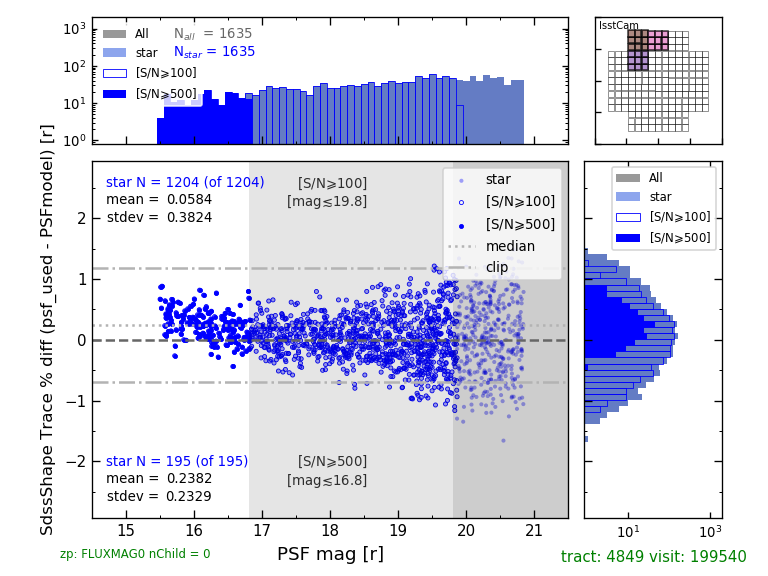
\includegraphics[width=0.8\textwidth]{plots/plot-v199540-psfTraceDiff-psfMagHist}
\caption{Brighter fatter effect evidence }
\label{fig:bfp}
\end{figure}



\subsubsection{Discussion}
We discussed how to implement change in code with tight turn around (need sign off from SciOps \gls{AD}).
How should one decide to rerun -  we need policies to affect or not nightly or daily changes in case of failures. Probably there is some percent level of problems we would accept, one percent seems ok two starts to seem a lot.  It was noted that problems stemming from a new software version should always have the possibility to revert to a previous stable version.

The need for some sort of rolled up \gls{QA} status were discussed - MacArthur came up with some summary files an example of which \texttt{visitAnalysis\_OpsRehearsal\_night1\_i.shortSum.txt} is in \appref{sec:visitsum}.


\subsection{Day 2} \label{sec:day2}

The daily meeting took place as planned at 11:00 \gls{PST}.

Transfers were initiated earlier than Day 1 with the 5 second delays removed, and all data had arrived at the \gls{LDF} by 7:30 am.
Data ingestion {\texttt{/project/OpsRehearsal\_1/night2} and processing were initiated shortly thereafter and were completed within roughly 1 hour.

No processing errors were reported, so examination of less severe issues were undertaken.
Noted were WARN-level problems that revolved around reference catalogs being in an outdated format
and the lack of zeropoint information for z- and Y-bands. 

\subsubsection{Discussion}
There were discussions about how the current \gls{pipeline}, operating on DC2 data might compare with what might
be needed during commissioning and operations.  
It was noted that because the rehearsal was using a processing \gls{pipeline} (and \gls{QA} tools) more amenable to \gls{Data Release Processing} (\gls{DRP}) that \gls{QA} products available might not be good comparisons to that needed when working with prompt processing.  
Also, it was noted that prompt processing \gls{QA} might form a basis for later selection of inputs to \gls{DRP}.

Another discussion revolved around whether WARN-level diagnostics might be dealt with in Operations/Commissioning.
Mostly it was felt that these fell into two classes:  those that were indicative of poor data (which might not require any intervention) and those that indicated software bugs (which should be tracked/resolved through tickets to the \gls{DM} developers).


\subsection{Day 3} \label{sec:day3}

The daily meeting took place as planned at 11:00 \gls{PST}.

Transfers were initiated similar to Day 2 and all data had arrived at the \gls{LDF} by 7:30 am.
Data ingestion {\texttt{/project/OpsRehearsal\_1/night3} required roughly 20 minutes.  
Processing was subsequently initiated but after 30 minutes it was found that jobs had never been submitte to the compute resource.  That resource (a reserved allocation) was found to still be running \gls{QA} from Night 2. An alternate compute resource was identified and jobs re-submitted, finishing $\sim$35 minutes later.

Similar WARN-level problems were identified prior to the daily meeting as were a 
small number of failures, similar to night 1 (number of stars resulting in failed \gls{PSF} modeling).

\subsubsection{Discussion}

Discussions centered on what information needed to be captured from this rehearsal for future rehearsals.
It was felt that this rehearsal proceeded relatively smoothly but did not include processes that could
mimic commissioning team's needs (i.e. fast turn around processing) and ad-hoc processing of data taken
to address specific tests.  The next rehearsal (late 2019/early 2020) is meant to focus toward 
LSST Commissioning with ComCam and should include Commissioning Team members.




\section{Conclusion and lessons learned}\label{sec:conc}
Though there were some limitations in out setup (\secref{sec:setup}) this was still useful exercise.

One central issue that should be followed-up on in subsequent rehearsals are the \gls{QA} metrics to be gathered during prompt processing and that utilities to provide rollups/summaries.

Though in the telecon status was discussed it was not properly recorded in the google sheet for the day,
there was no designated minute taker an individuals did not necessarily add a summary. In operations such a status
report should probably be filled even before the meeting.





\appendix

\section{sec:visitsum}
\begin{code}
\begin{code}
# Stars: Mag(Gaussian) - PSFMag (mmag) (commonZP)
#                filter    mean    stdev    median     num      numTot  NumEntries
# straight avg       i    -0.46     6.84    -0.56     51258     52230        83
# weighted avg       i    -0.43     6.67    -0.52     51258     52230        83
#================================================================================
# Stars: Mag(CircAper12pix) - PSFMag (mmag) (commonZP)
#                filter    mean    stdev    median     num      numTot  NumEntries
# straight avg       i    -1.08     9.63    -1.20     51373     52230        83
# weighted avg       i    -1.05     9.57    -1.16     51373     52230        83
#================================================================================
# Stars: Mag(Gaussian) - PSFMag (mmag)
#                filter    mean    stdev    median     num      numTot  NumEntries
# straight avg       i    -0.46     6.84    -0.56     51258     52230        83
# weighted avg       i    -0.43     6.67    -0.52     51258     52230        83
#================================================================================
# Stars: Mag(CircAper12pix) - PSFMag (mmag)
#                filter    mean    stdev    median     num      numTot  NumEntries
# straight avg       i    -1.08     9.63    -1.20     51373     52230        83
# weighted avg       i    -1.05     9.57    -1.16     51373     52230        83
#================================================================================
# Stars:   SdssShape Trace (calib_psf_used): $\sqrt{0.5*(I_{xx}+I_{yy})}$ (pixels)
#                filter    mean    stdev    median     num      numTot  NumEntries
# straight avg       i     1.50     0.01     1.50     39435     39441        83
# weighted avg       i     1.51     0.01     1.51     39435     39441        83
#================================================================================
# Stars:  SdssShape Trace: $\sqrt{0.5*(I_{xx}+I_{yy})}$ (pixels)
#                filter    mean    stdev    median     num      numTot  NumEntries
# straight avg       i     1.51     0.01     1.51     51513     52230        83
# weighted avg       i     1.51     0.01     1.51     51513     52230        83
#================================================================================
# Stars:  SdssShape Trace % diff (psf_used - PSFmodel)
#                filter    mean    stdev    median     num      numTot  NumEntries
# straight avg       i     0.05     0.54     0.06     39411     39441        83
# weighted avg       i     0.03     0.52     0.05     39411     39441        83
#================================================================================
# Stars: PSF - ref (calib_psf_used) (mmag)
#                filter    mean    stdev    median     num      numTot  NumEntries
# straight avg       i     1.08     7.07     1.12     36861     37100        83
# weighted avg       i     1.04     7.04     1.08     36861     37100        83
#================================================================================
# Stars:  PSF - ref (calib_photom_used) (mmag)
#                filter    mean    stdev    median     num      numTot  NumEntries
# straight avg       i     1.30     7.58     1.26     48957     49377        83
# weighted avg       i     1.27     7.55     1.23     48957     49377        83
#================================================================================
# Stars: PSF - ref (mmag)
#                filter    mean    stdev    median     num      numTot  NumEntries
# straight avg       i     1.26     7.60     1.24     50483     50939        83
# weighted avg       i     1.23     7.56     1.19     50483     50939        83
#================================================================================
# Stars: CircAper12pix - ref (calib_psf_used) (mmag)
#                filter    mean    stdev    median     num      numTot  NumEntries
# straight avg       i     0.41     7.33     0.35     35636     37100        83
# weighted avg       i     0.41     7.32     0.34     35636     37100        83
#================================================================================
# Stars:  CircAper12pix - ref (calib_photom_used) (mmag)
#                filter    mean    stdev    median     num      numTot  NumEntries
# straight avg       i     0.28     7.41     0.22     47018     49377        83
# weighted avg       i     0.29     7.39     0.22     47018     49377        83
#================================================================================
# Stars: CircAper12pix - ref (mmag)
#                filter    mean    stdev    median     num      numTot  NumEntries
# straight avg       i     0.20     7.50     0.12     48218     50939        83
# weighted avg       i     0.20     7.48     0.12     48218     50939        83
#================================================================================
# Stars: matches_distance_calib_astrometry_used (mas)
#                filter    mean    stdev    median     num      numTot  NumEntries
# straight avg       i     7.51     4.51     6.70     50403     50939        83
# weighted avg       i     7.51     4.50     6.72     50403     50939        83
#================================================================================
# Stars: matches_distance (mas)
#                filter    mean    stdev    median     num      numTot  NumEntries
# straight avg       i     7.51     8.76     6.70     50403     50939        83
# weighted avg       i     7.51     8.76     6.72     50403     50939        83
#================================================================================
# Stars:  $\delta_{Ra}$ = $\Delta$RA*cos(Dec) (mas) (calib_astrom_used)
#                filter    mean    stdev    median     num      numTot  NumEntries
# straight avg       i    -0.02     7.04    -0.08     50781     50939        83
# weighted avg       i     0.01     7.05    -0.06     50781     50939        83
#================================================================================
# Stars: $\delta_{Ra}$ = $\Delta$RA*cos(Dec) (mas)
#                filter    mean    stdev    median     num      numTot  NumEntries
# straight avg       i    -0.02     7.04    -0.08     50781     50939        83
# weighted avg       i     0.01     7.05    -0.06     50781     50939        83
#================================================================================
\end{code}

\end{code}

% Include all the relevant bib files.
% https://lsst-texmf.lsst.io/lsstdoc.html#bibliographies
\label{sec:bib}
\bibliography{lsst,lsst-dm,refs_ads,refs,books}

%Make sure lsst-texmf/bin/generateAcronyms.py is in your path
%\section{Acronyms used in this document}\label{sec:acronyms}
%\addtocounter{table}{-1}
\begin{longtable}{|l|p{0.8\textwidth}|}\hline
\textbf{Acronym} & \textbf{Description}  \\\hline

AD & Associate Director \\\hline
CCD & Charge-Coupled Device \\\hline
DESC & Dark Energy Science Collaboration \\\hline
DM & Data Management \\\hline
DMTN & \gls{DM} Technical Note \\\hline
DRP & Data Release Production \\\hline
DTN & Data Transfer Node \\\hline
FIU & Florida International University \\\hline
LDF & \gls{LSST} Data Facility \\\hline
LDM & \gls{LSST} Data Management (Document Handle) \\\hline
LSST & Large Synoptic Survey Telescope \\\hline
NCSA & National Center for Supercomputing Applications \\\hline
PSF & Point Spread Function \\\hline
PST & Project Science Team \\\hline
QA & Quality Assurance \\\hline
\end{longtable}

%Unccomment these if you want old style acronyms
\label{sec:acronyms}
\printglossaries

\end{document}
